%!mode::"TeX:UTF-8"
\documentclass{ctexart}
\usepackage{amsmath}
\usepackage{amssymb}
\usepackage{xltxtra}
\usepackage{mflogo,texnames}
\usepackage{graphicx}
\usepackage{listings}
\usepackage{listing}
\usepackage{xcolor}
\usepackage{xcolor}
\usepackage{enumerate}
\usepackage[colorlinks,linkcolor=blue]{hyperref}
\usepackage{cite}
\usepackage{color}
\usepackage{caption}
\usepackage{subfigure}
\usepackage[top=2.54cm,bottom=2.54cm,left=3.18cm,right=3.18cm]{geometry}
\author{右武卫大将军}
\title{使用文本挖掘和情感分析对在线论坛的热点进行侦测和预测}
\begin{document}
    \maketitle
    \section{摘要}
        文本情感分析或者叫做情感极性计算已经成为了文本挖掘领域的最受关注的前言领域。本文研究的是使用情感分析和文本挖掘的办法来对论坛热点进行探测和预测。首先,我们设置一个可以自动计算文本极性的算法,然后为每一个文本进行评分。第二,将该方法和K 均值聚类,SVM 算法相结合,拓展为一种非监督的文本挖掘方法。我们使用这种文本挖掘办法将论坛文本划分到不同的聚类组中,每一组的中心代表着当前的一个论坛热点,这些组涵盖了31 个不同的论坛话题和220053 张帖子。实验结果表明结合了K- 均值聚类方法的SVM 算法的预测结果具有很强的一致性。由SVM 计算出来的排名前十的论坛热点涵盖了K 均值聚类80\% 的结果。对于本年的数据,SVM 和K 均值在排名前4 的论坛热点上具有完全的一致性。
    \section{介绍}
        在互联网和信息化时代,在线数据量会指数级膨胀。这些网页数据主要的存在方式就是非结构化的文本,很难自动处理。不同于静态网页,非结构化的或者松散的结构化文本常以各种有形的,或者无形的动态交互网站上出现。各种各样的社区,网站,论坛构成了今天的交互式互联网。但面对来自于各种线上论坛的海量在线信息,信息搜寻者很难确定哪一些信息是有用。这促使研究者去研究如何识别在线论坛的中心热点,这样就可以快速锁定互联网上的核心信息。我们的研究提供了一种容易理解又及时的关于不同论坛的有趣的结构性的自然群组分析,这一分析可以动态的追踪论坛中的热点,从而促进互联网社群网络中的成员更好的做决策。

        正如高效的商业智能分析方法,数据挖掘和机器学习方法提供了众多工具可以动态处理大量线上数据。另一个最近发展起来的叫做情感分析(也叫情绪极性计算)的方法也已经应用于线上文本挖掘领域。文本情感分析的目标是计算出发布人在某一特定话题下的态度。这一态度可以是任何形式的评断,评估或者情绪状态。公认之下,情感分类算法的性能是与特定话题领域相关联的。

        本论文中,线上论坛热点追踪和预测涉及到了情感分析和文本挖掘方法。我们分两个阶段来研究这一问题:情感极性计算和基于K 均值聚类与SVM 算法的聚合情感分析。这一无监督的文本挖掘方法会将论坛文本分组到不同的聚类组别中,每一个聚类组的中心点代表当前时间段的一个论坛热点中心。数据收集自新浪运动论坛,这一论坛有31 个不同的主题和220053 个帖子。在同一个时间窗口内的计算结果表明,SVM 的预测结果和K 均值聚类有极大的相似性。

        本文剩余部分的结构安排如下:第二节会讨论与本文相关的其他研究工作,第三节提出模型和方法论,第四节会讨论实证研究结果和相关讨论,最后第四节也会对论文进行总结。

    \section{相关工作}
        这一节总结了三个相关研究的发展历程:线上论坛的动态聚类分析,线上文本的情感分析和使用机器学习方法对线上文本挖掘。

        \subsection{线上论坛的动态聚类分析}
            由于以下两个原因线上论坛彼此关联起来。第一,论坛上传播的热点公共事件都有着相似的主题。比如说,在一个娱乐社群中,学院派颁奖论坛和金球奖颁奖论坛高度相关。第二,新兴的事件会在某些特定的论坛之间建立起临时得关联。比如说电影(No Country For Old Men)在2008 年的学院派评选中获得了最佳动作片奖项,这件事在Oscar 颁奖期间将相关的论坛都连接在一起。我们的目标是研究第二种论坛内部的连接,并且提出一种数学机制可以动态的捕获,描述并预测这些随时间变化的相关关系。

            有很多论文研究过多种多样的交互式社会网络,比如个人动态网络,工业制造者动态网络,企业动态网络,线上虚拟社群动态网络。该领域第一篇重要文献是Asavathiratham 在MIT 完成的博士论文(1996)创造了一个影响模型作为网络马尔科夫链动态性的一个简单表示。这一工作被很多学者所引用,比如用于自动学习基于可穿戴设备传感器的人群分组的社会网络结构。文献【34】 选择了662 家广东佛山的陶器制造厂进行聚类来构造一个竞争关系网络(Competition Relationship Network,CRN),并证明了通过竞争关系构建的网络是一个和规模无关的高度聚类的网络。并且,在股票市场上的相关企业网络也是一个重要的研究领域。将线上虚拟社区看成是动态的,这就提出了一个关系代数方法可以用来解决虚拟社区网络上的计算问题。

            实际上,关于线上运动论坛的实时动态性的刻画还是比较少的。一个虚拟社区中的线上运动论坛是我们研究的目标,其中会使用机器学习的办法来动态刻画内部结构,并根据情感极性来对论坛内容进行聚类。

        \subsection{对web页面进行情感分析}
            对文本进行分类的标准有很多,比如话题,结构,作者,时代等等。基于情感极性的文本分类成为了吸引网页挖掘社区的一个新的研究方向。为了说明它的工作原理,假设你想去C 城市度假,你可能会用到一个搜索引擎来搜索C 城市的相关信息。如果能够知道有多大比例的返回结果推荐C 城市作为旅游目的地,这便是一个有用的信息。将情感分析和搜索引擎以及文本检索技术合并在一起可以为用户提供更有效率和功能的服务。情感分析已经大量应用于新闻推荐和总结,在线论坛,文件分享或者聊天室等等应用之上。YouTube 在今年年初引入了情感分类功能来对所有的评论分组为“Poor” 或者“Good”。

            作为一个极具前景的研究领域,文本情感分析已经被深入研究过,并作为文本分类的辅助工具。已有的情感计算方法分为两种类型,一种是基于机器学习方法的,一种是基于语义方法的。深入研究过的语言包括英语,汉语以及阿拉伯语。本文的目标是进一步延伸文本情感分析,将其引入到线上论坛内容的动态聚类当中,初步的测试论坛是一个中文运动论坛。

        \subsection{基于机器学习的文本挖掘}
            为了对论坛的热点进行聚类和预测,我们使用两种机器学习方法(K均值和SVM)。K均值和SVM 方法在各种应用当中被广泛使用。在我们的研究当中,机器学习是情感极性分析和网络动态性分析的中间桥梁。新浪体育社区中的所有子论坛构成了我们研究的总体目标,其中每一个子论坛都会被转换成一个向量,来代表在当前时间窗口用户的注意力,转换的原则包括帖子的数量以及相应的情感得分平均值。由特征工程所构造的这些向量会填喂给机器学习算法用于聚类和预测。

    \section{模型和方法论}
        本文的方法可以被简述为以下步骤:数据收集和清洗,文本的情感分析,基于K 均值聚类的热点事件检测,最后是基于SVM 方法的热点事件预测。图\ref{fig_1} 说明了整篇文章的方法,其中用三个模型来把文本情感分析,K 均值聚类,和SVM 拼接在一起来分析论坛里的热点事件。
        \begin{figure}[hb]
            \centering
            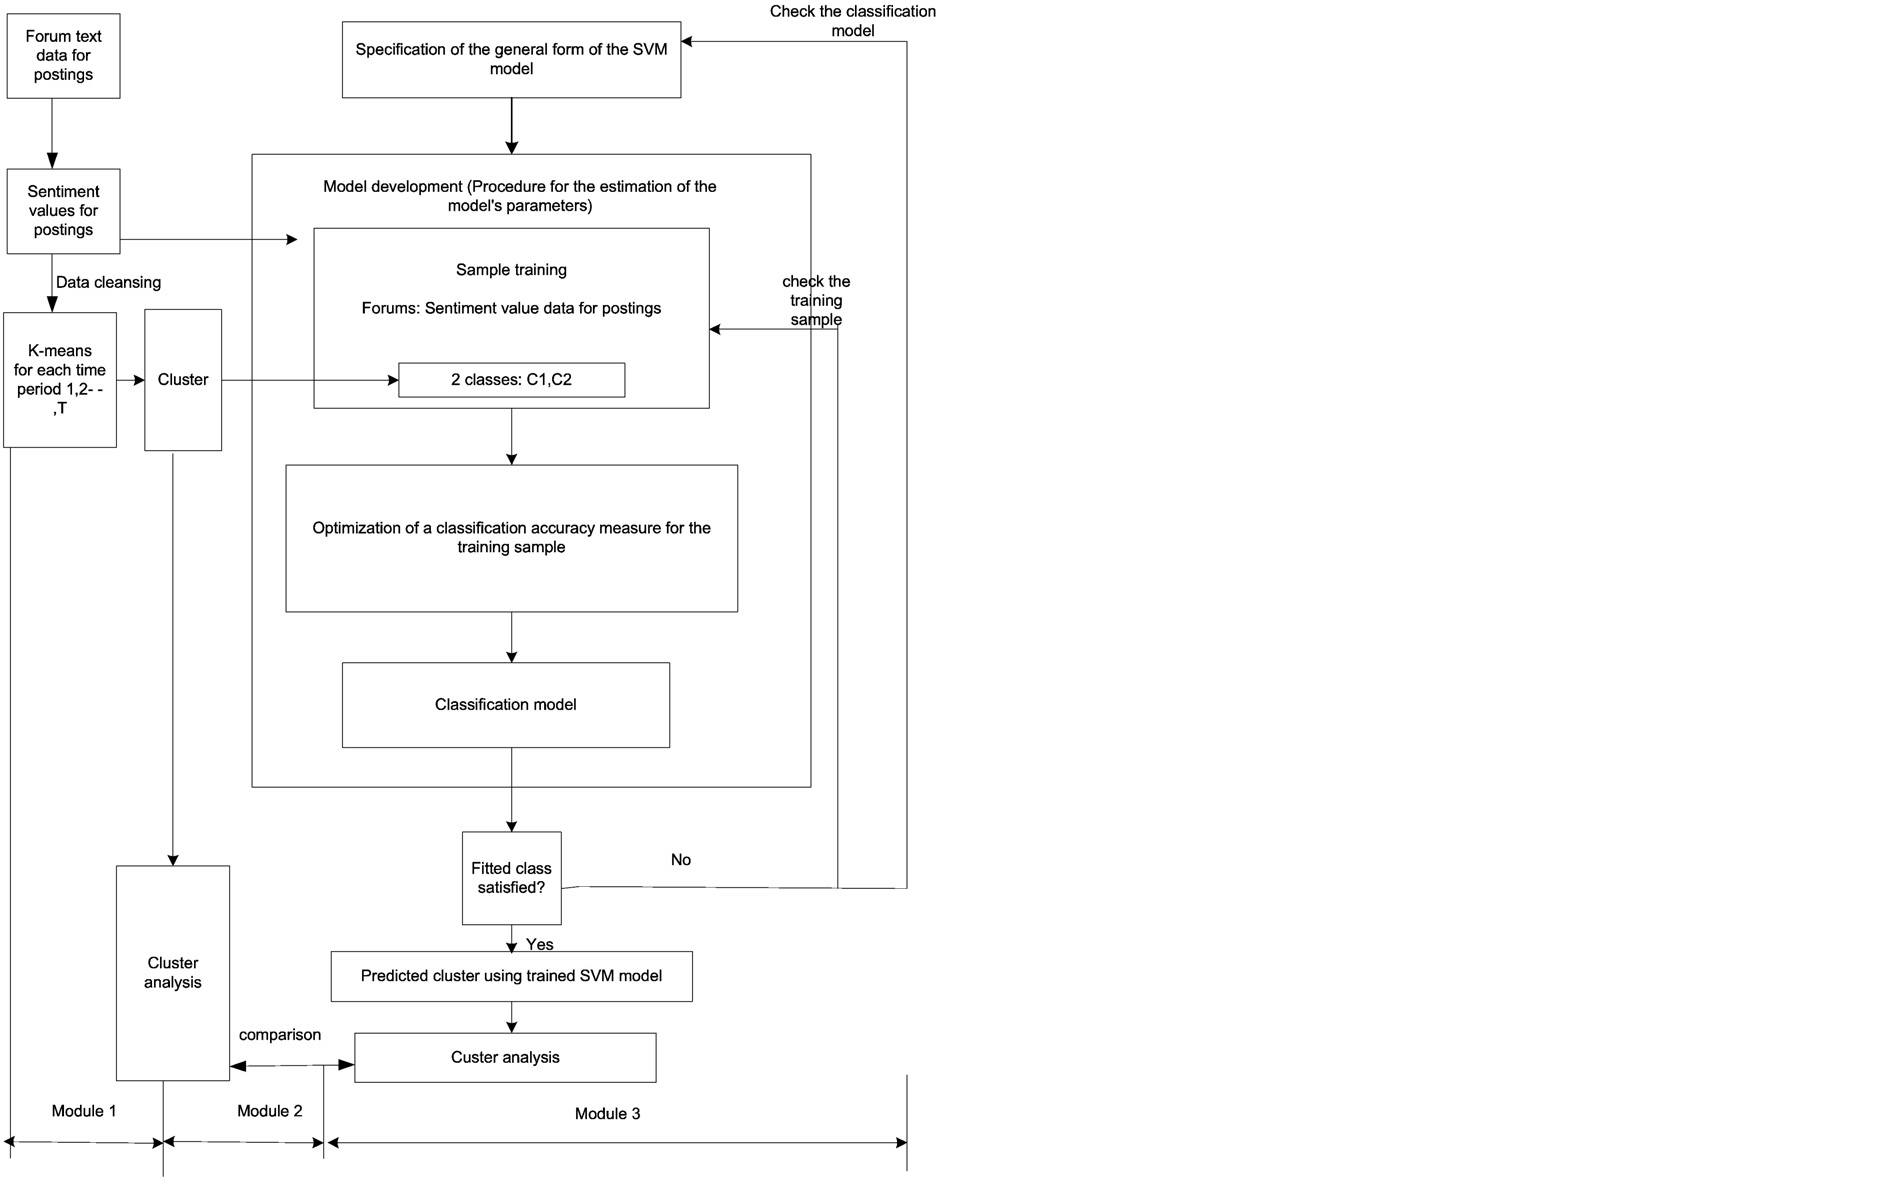
\includegraphics[width=1.1\textwidth]{fig_1}
            \caption{本文方法的图示}
            \label{fig_1}
        \end{figure}

        模型1使用文本情感计算和分析的办法将中文文本转换为一个向量。在本模型中,通过使用特定的商业工具实现一种基于关键词的方法来对每一段文本计算情感得分。每一个帖子会得到一个整型的分数,它的符号代表情感的极性,而它的值代表情感的强度。基于模型1所得出的情感分数,模型2会使用K均值算法将新浪运动论坛社区的帖子按时期进行聚类。在K均值算法中有五个输入特征,帖子的数量,帖子的平均回复数量,帖子的平均情感得分,正向情绪的帖子比率和负向情绪的帖子比率。热点子论坛就可以通过K均值的方法进行识别,即那些聚类的中心点(子论坛)。这一方法基本上是延续前人的方法。模型2是基于SVM的分类模型,它首先利用子论坛相关信息构成进行聚类分析,其结果构成训练数据,对SVM进行训练,然后使用训练好的SVM模型对热点子论坛进行识别。本文使用的方法与之前的情感分析的方法,无论是基于机器学习的还是语义分析的,都有所不同。实际上,我们将语义分析和机器学习的方法聚合在一起,并进一步将文本情感分析延伸到聚类分析,以便于分析线上社区的网络动态性。
        
        \subsection{数据收集}
            在开始数据爬取和清洗之前,很有必要提前了解一下新浪运动社区的基本结构。新浪线上运动社区构成了一个树状结构,有根论坛,有分支论坛,有不再分割的叶子论坛。这里总共有49个子论坛。图\ref{fig_2}展现了该网站的完整树状结构。
            \begin{figure}[hb]
                \centering
                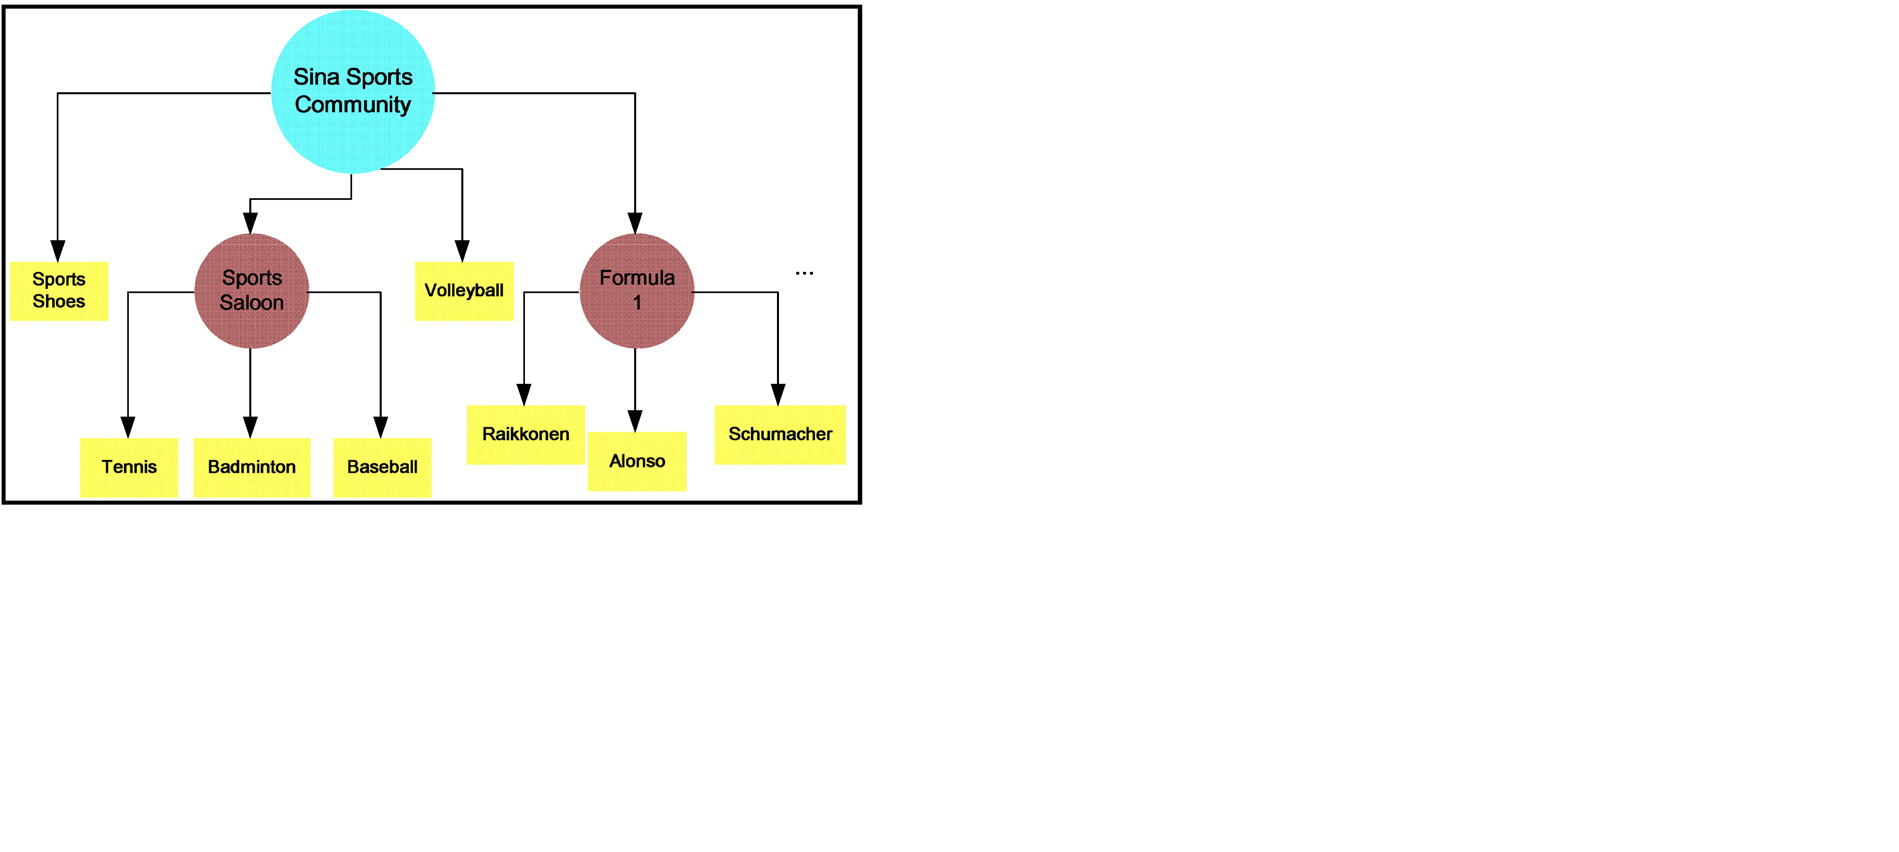
\includegraphics[width=1.1\textwidth]{fig_2}
                \caption{新浪线上运动社区基本结构}
                \label{fig_2}
            \end{figure}
            
            
            


\end{document}
